% !TeX root = ../main.tex

\section{Z transform}
\begin{LARGE}
    $$
    X(z)=\sum_{n=-\infty}^{+\infty}x(n)\cdot z^{-n}
    $$
    $$
    z=\rho e^{j2\pi f}
    $$ 
\end{LARGE}

\subsection{Complex Numbers Fundamentals}
\begin{LARGE}
    $$
    \cos x=\frac{
        e^{jx}+e^{-jx}
    }{2}\qquad
    \sin x=\frac{
        e^{jx}-e^{-jx}
    }{2j}
    $$
    $$
    z=\rho e^{\pm j\theta}=\rho(\cos(\pm\theta)+j\sin(\pm\theta))
    $$
    $$
    |z|=\sqrt{Re(z)^2+Im(z)^2}=\rho
    $$
\end{LARGE}


\subsection{Notable transforms}
An example
$$x(n)=\delta(n)+\delta(n+1)+2\delta(n-2)$$
$$X(z)=1+z+2z^{-2}$$
\begin{itemize}
    \item $Z\brackets{\delta(n-k)}=z^{-k}$, a delay of $k$ samples
    \item $Z\brackets{x(n-k)}=X(z)z^{-k}$
    \item $Z\brackets{a^nu(n)}=\frac{1}{1-az^{-1}}$, discrete exponential term
    \item $Z\brackets{ax(n)+by(n)}=aX(z)+bY(z)$
    \item $Z\brackets{x(-n)}=X(z^{-1})$
    \item $Z\brackets{nx(n)}=-z\frac{dX(z)}{dz}$
    \item $Z\brackets{x(n)*y(n)}=X(z)\cdot Y(x)$, convolution theorem
    \item $Z\brackets{-a^nu(n)}=\frac{1}{1-z^-1}$, unitary step
    \item $Z\brackets{r^n\cos(\omega_0n)u(n)}=\frac{1-r\cos(\omega_0)z^{-1}}{1-2r\cos(\omega_0)z^-1+r^2z^{-2}}$
\end{itemize}

\subsection{Z transform expressions}
\begin{enumerate}
    \item 
    \begin{LARGE}
        $$
        X(z)=\frac{N(z)}{D(z)}=\frac{
            b_0+b_1z^{-1}+\cdots b_Nz^{-N}
        }{
            a_0+a_1z^{-1}+\cdots+a_Dz^{-D}
        }
        $$
    \end{LARGE}
    Useful to compute the inverse Z transform
    \item
    \begin{LARGE}
        $$
            X(z)=z^{D-N}\frac{b_0}{a_0}\frac{
                \prod_{i=1}^N(z-z_i)
            }{\prod_{i=1}^D(z-p_i)}
        $$
    \end{LARGE}
    Useful for filter characterization
\end{enumerate}

\subsection{Z transform relationship with LTI systems}
Given $x(n)$ and $h(n)$ (impulse response of LTI system)
$$y(n)=x(n)*h(n)$$
The same system can also be described by a linear difference equation with constant coefficients
    $$
    \sum_{k=1}^Da_ky(n-k)=
    \sum_{k=0}^Nb_kx(n-k)
    $$
    $$
    y(n)=\underlabel{\sum_{k=0}^Nb_kx(n-k)}{Moving Average (FIR)}-
    \underlabel{\sum_{k=1}^Da_ky(n-k)}{Autoregressive, feedback (IIR)}
    $$
Converting in Z domain
    $$
    \sum_{k=1}^Da_ky(n-k)=
    \sum_{k=0}^Nb_kx(n-k)
    $$
    $$
    Y(z)\sum_{k=0}^Da_kz^{-k}=
    X(z)\sum_{k=0}^Nb_kz^{-k}
    $$
As $Y(z)=X(z)H(z)$
$$
H(z)=\frac{Y(z)}{X(z)}=\frac{\sum_{k=0}^Nb_kz^{-k}}{\sum_{k=0}^Da_kz^{-k}}
$$
At denominator IIR part

\subsection{Inverse Z transform}
$$
H(z)=\frac{Y(z)}{X(z)}=\frac{\sum_{k=0}^Nb_kz^{-k}}{\sum_{k=0}^Da_kz^{-k}}
$$
Given
$$
H(z)=\sum_{n=0}^kh(n)z^{-n}
$$
We can compute its root decomposition
$$
H(z)=h_0\prod_{n=1}^k(1-z_nz^{-1})\qquad h_0=H(n=0)
$$
$z_n$ are called roots of the polynomial $H(z)$. Thanks to convolution theorem
$$
H(z)=h_0\cdot H_1(z)\cdot H_2(z)\cdots H_k(z)
$$
$$
\Downarrow
$$
$$
h(n)=h_0\cdot h_1(n)*h_2(n)*h_3(n)*\cdots*h_k(n)
$$
Where
$$
h_i(n)=Z^{-1}\brackets{1-z_iz^{-1}}=\delta(n)-z_1\delta(n-1)
$$

\subsection{Partial fract expansion for computing $Z^{-1}$}
\begin{LARGE}
    $$
    H(z)=\frac{Y(z)}{X(z)}=\frac{\sum_{k=0}^Nb_kz^{-k}}{\sum_{k=0}^Da_kz^{-k}}
    =
    \sum_{k=1}^D\sum_{m=1}^M\frac{
        r_{k_m}
    }{(1-p_kz^{-1})^m}+
    \underlabel{
        \sum_{k=0}^{N-D}c_kz^{-k}
    }{$N\geq D$}
    $$
\end{LARGE}
$M$ is the multiplicity of the root (or pole) $p_k$. The Z transform inversion is the sum of simple inversions (causal):
\begin{itemize}
    \item $Z^{-1}\begin{Bmatrix}
        \frac{r_{k_1}}{(1-p_kz^{-1})}
    \end{Bmatrix}=r_{k_1}\cdot (p_k)^nu(n)$
    \item $Z^{-1}\begin{Bmatrix}
        \frac{r_{k_2}}{(1-p_kz^{-1})^2}
    \end{Bmatrix}=r_{k_2}\cdot (n+1)(p_k)^nu(n)$
    \item $Z^{-1}\Brackets{c_kz^{-k}}=c_k\cdot \delta(n-k)$
\end{itemize}

\subsection{Zeros-Poles factorization}
\begin{LARGE}
    $$
    H(z)=\frac{
        \sum_{k=0}^Nb_kz^{-k}
    }{\sum_{k=0}^Da_kz^{-k}}
    =z^{D-N}\frac{b_0}{a_0}\frac{
        \prod_{i=1}^N(z-z_i)
    }{\prod_{i=1}^D(z-p_i)}
    $$
\end{LARGE}
\begin{itemize}
    \item For a system to be stable
    $$
    \sum_{n=-\infty}^\infty|h(n)|<\infty
    $$
    If instable output of the system goes to the infinite
    \item If all poles of the $H(z)$ are inside the unitary circle ($|p_i|<1\,\,\forall\,\,i$) the system is stable
    \item If one positive zero is inside the unitary circle, it is called minimum phase
    \item If one positive zero is outside the unitary circle, it is called maximum phase
    \item \textbf{It is FIR if there is no denominator}
    \item \textbf{It is IIR if there is feedback $y=y...$}
\end{itemize}
\textbf{To move from maximum phase to minimum phase, consider the reciprocals of the zeros}.

\subsubsection{Transfer function evaluation in time domain: direct form \#1}
\begin{center}
    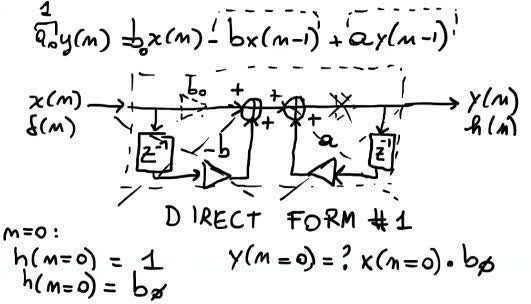
\includegraphics[width=0.8\textwidth]{images/Screenshot from 2022-10-07 16-24-14.png}
\end{center}
Direct form \#1, in this case for $n<0$ the system for us it does not exist, so zero: so $h(n=0)=b_0=1$ in our case

\subsubsection{From generic output to transfer function and complex conjugates}
Consider
$$
y(n)=0.5x(n)-2x(n-1)+x(n-2)-2\rho\cos(\theta)y(n-1)-\rho^2y(n-2)
$$
We can easily find $H(z)$, the coefficients of the $y$ on the right must change sign as they go to the left:
$$
H(z)=\frac{
    0.5-2z^{-1}+z^{-2}
}{
    1+2\rho\cos(\theta)z^{-1}+\rho^2z^{-2}
}
$$
Also $h(n=0)=b_0=0.5$ and $y(n=0)=x(n=0)\cdot 0.5$

The $1+2\rho\cos(\theta)z^{-1}+\rho^2z^{-2}$ represents 2 complex conjugates:
$$
1-2\rho\cos(\theta)z^{-1}+\rho^2z^{-2}\rightarrow \rho(\cos(\theta)\pm j\sin(\theta))
$$
$
1+2\rho\cos(\theta)z^{-1}+\rho^2z^{-2}\rightarrow -\rho e^{\pm j\theta}
\\
1-2\rho\cos(\theta)z^{-1}+\rho^2z^{-2}\rightarrow \rho e^{\pm j\theta}
$

Their product is a real coefficient!

\textbf{In general if the numerator and the denominator are expressed with $z^{-1}$, solve them normally (imposign $z^{-1}=w$ and then invert the results) or exploiting the above formulas then introduce a number of zeros (if solved the denominator) or poles (if solved the numerator) equal to the maximum grade of the polynomial, which will simplify}.

\subsubsection{Maximum phase to minimum phase}
$$
H(z)=h_0+h_1z^{-1}+\cdots+h_Nz^{-N}\Leftrightarrow G(z)=z^{-N}H^*(z^{-1})
$$
The $G$ version will have the same coefficients but in reverse order and \textbf{exact same magnitude}

The roots that are maximum phase will become minimum phase by choosing their reciprocal in conjugate position, an example:
$$
H_M(z)=\frac{
    \left(
        1-2\sqrt{2}z^{-1}+4z^{-2}
    \right)
    \left(
        1+2\sqrt{2}z^{-1}+4z^{-2}
    \right)
}{4+z^{-2}}
$$
The numerator (only it) introduce maximum phase, write their $G$ version:
$$
H_m(z)=\frac{
    \left(
        4-2\sqrt{2}z^{-1}+z^{-2}
    \right)
    \left(
        4+2\sqrt{2}z^{-1}+z^{-2}
    \right)
}{4+z^{-2}}
$$
Alternatively
As $\rho=2$, now $\rho=\frac{1}{2}$:
$$
H_m(z)=A\frac{
    \left(
        1-\frac{\sqrt{2}}{2}z^{-1}+\frac{1}{4}z^{-2}
    \right)
    \left(
        1+\frac{\sqrt{2}}{2}z^{-1}+\frac{1}{4}z^{-2}
    \right)
}{4+z^{-2}}
$$

\subsection{All-pass filter}
It has this form:
$$
H(z)=\frac{c+z^{-1}}{1+cz^{-1}}
$$
\textbf{Has magnitude constant=1, keeps magnitude and changes the phase}. To achieve it place the pole in a reciprocal conjugate position w.r.t. zero (if zero in 2, put pole in $\frac{1}{2}$)
$$
y(n)=cx(n)+x(n-1)-cy(n-1)
$$
More in general it has this form:
$$
H(z)=\frac{
    a_0+a_1z^{-1}+\cdots+a_{n-1}z^{n-1}+a_nz^{-n}
}{
    a_n+a_{n-1}z^{-1}+\cdots+a_1z^{n-1}+a_0z^n
}
$$